% generated by scripts/pkl_to_latex.py
% source PKL : vscan_v1_L6_Ne4_U10_t1_mode-uniform_nmin2_solver-gcg_sz0_restarts10_iter300_kmax4_tol1em09_V0to15_N16-2f7c06936fa2.pkl
% scan type  : vscan
% state      : gs
% requires   : \usepackage{pgfplots} \pgfplotsset{compat=1.18}
% colours match the matplotlib PDF (tab10 cycle)
\definecolor{gmeC0}{HTML}{1F77B4}
\definecolor{gmeC1}{HTML}{FF7F0E}
\definecolor{gmeC2}{HTML}{2CA02C}
\definecolor{gmeC3}{HTML}{D62728}
\definecolor{gmeC4}{HTML}{9467BD}
\definecolor{gmeC5}{HTML}{8C564B}
\definecolor{gmeC6}{HTML}{E377C2}
\definecolor{gmeC7}{HTML}{17BECF}

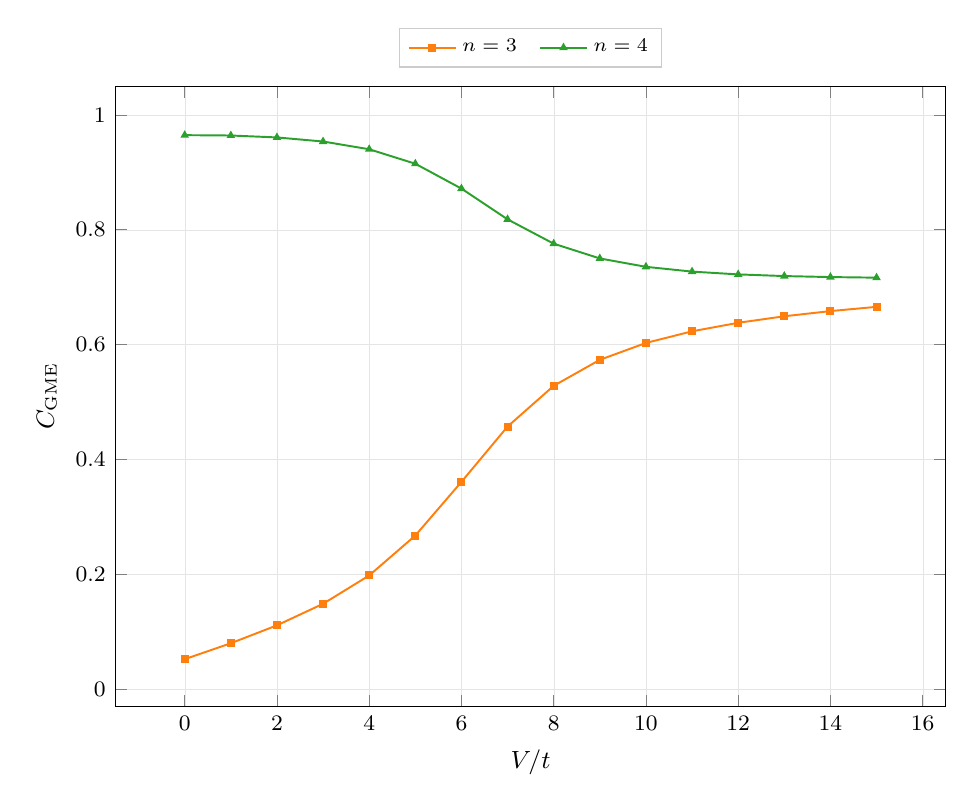
\begin{tikzpicture}
  \begin{axis}[
    width=\columnwidth,
    height=0.78\columnwidth,
    xlabel={$V/t$},
    ylabel={$C_{\mathrm{GME}}$},
    grid=both,
    grid style={line width=.1pt, draw=gray!20},
    tick label style={font=\footnotesize\rmfamily, /pgf/number format/fixed},
    label style={font=\small\rmfamily},
    scaled ticks=false,
    legend style={font=\scriptsize\rmfamily, draw=gray!40, at={(0.5,1.03)}, anchor=south, /tikz/every even column/.append style={column sep=6pt}},
    legend cell align={left},
    legend columns=2,
    ymin=-0.03,
    ymax=1.05,
  ]
    \addplot[color=gmeC1, mark=square*, mark size=1.1pt, line width=0.7pt] coordinates {
        (0,0.052128) (1,0.079859) (2,0.111046) (3,0.148563)
        (4,0.197909) (5,0.267413) (6,0.360887) (7,0.457222)
        (8,0.528143) (9,0.573395) (10,0.602784) (11,0.623067)
        (12,0.637903) (13,0.649271) (14,0.658301) (15,0.665675)
    };
    \addlegendentry{$n=3$}
    \addplot[color=gmeC2, mark=triangle*, mark size=1.1pt, line width=0.7pt] coordinates {
        (0,0.964641) (1,0.964053) (2,0.960703) (3,0.953585)
        (4,0.94011) (5,0.914889) (6,0.871593) (7,0.818035)
        (8,0.775684) (9,0.749962) (10,0.735379) (11,0.727049)
        (12,0.722179) (13,0.719276) (14,0.717531) (15,0.716491)
    };
    \addlegendentry{$n=4$}
  \end{axis}
\end{tikzpicture}
